\documentclass{beamer}
\usepackage{graphicx}
\usepackage{listings}
\usepackage{xcolor}
\usepackage{amsmath, amssymb, amsthm, amsfonts}

\usetheme{CambridgeUS}
\usecolortheme{dolphin}
\setbeamertemplate{navigation symbols}{}
\setbeamertemplate{footline}[frame number]
\setbeamertemplate{frametitle}[default][center]

\lstdefinelanguage{Coq}{
  morekeywords={
    Definition, Theorem, Proof, Qed, Lemma, Inductive, Record, Fixpoint, 
    Module, Import, Require, Export, Module, End, Variable, Hypothesis,
    Parameter, Parameters, Variables, Axiom, Axioms, Section, Context,
    Contextual, Goal, Abort, Admitted, Unset, Set, Generalizable, Universes, 
    Instance, Class, Structure, Canonical, CoInductive, Variant, CoFixpoint, 
    Hypotheses, Assumption, Parameter, Ltac, with, Definition, Print,
    Declare, Scope, Arguments, Transparent, Opaque, Equations, CoFix, 
    Scheme, Mutual, Unset, Strategy, Elimination, Inversion, Inversion_clear,
    forall, exists
  },
  sensitive=true,
  morecomment=[s]{(*}{*)},
  morestring=[b]",
}

\lstset{
  language=Coq,                        % Specify the language
  basicstyle=\ttfamily\small,          % Set the font style and size
  keywordstyle=\color{blue},           % Color for keywords
  commentstyle=\color{gray},           % Color for comments
  stringstyle=\color{red},             % Color for strings
  numbers=left,                        % Line numbers on the left
  numberstyle=\tiny\color{gray},       % Style for line numbers
  stepnumber=1,                        % Line number increment
  numbersep=10pt,                      % Distance between code and line numbers
  showstringspaces=false,              % Don't show spaces in strings
  breaklines=true,                     % Automatic line breaking
  frame=single,                        % Frame around the code block
  captionpos=b,                        % Position of the caption
}

\title{The Quite Reasonable Effectiveness of 
Formalization in Programming Language Design}
\author{Jamie Fulford\\Advisors: Steve Zdancewic, Stephen Mell}
\institute[Penn]{
  Department of Computer and Information Science\\
  The University of Pennsylvania
}
\date[REPL 2024]{REPL, August 2, 2024}

\begin{document}

% Introduction here
% Make it clear that I've only been in PL for a few months
% so some ideas I present may seem obvious to some of you
% but hopefully to the rest of you they will be new and interesting
\frame{\titlepage}

% Argue that we are going to find a similar analogy for formalization
% Argue that it is like "effictively calculable"
\begin{frame}{"Quite Reasonable Effectiveness"}
  \begin{columns}
    \begin{column}{0.5\textwidth}
      \begin{itemize}
        \onslide<3->
        \item Eugene Wigner's "Unreasonable Effectiveness of Mathematics in the Natural Sciences"
        \onslide<4->
        \item What is reasonable effectiveness?
        \onslide<5->
        \item Reasonable effectiveness as a measure of utility
      \end{itemize}
    \end{column}
    \begin{column}{0.5\textwidth}
      \begin{figure}
        \onslide<2->
        \centering
        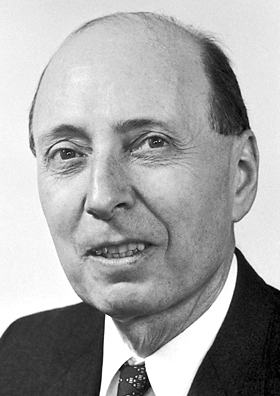
\includegraphics[height=0.6\textheight]{wigner}
      \end{figure}
    \end{column}
  \end{columns}
\end{frame}

% Define formalization quickly then talk about what makes it hard
\begin{frame}{The Experience of Formalization}
  \pause
  \begin{itemize}
    \item Expection: Proofs are hard
    \pause
    \item Reality: Proofs are easy, \textit{definitions} are hard
    \pause
    \item "Premature optimization is the root of all evil."
  \end{itemize}
\end{frame}

\begin{frame}{The Experience of Formalization}
  \begin{itemize}
    \item Expection: Proofs are hard
    \item Reality: Proofs are easy, \textit{definitions} are hard
    \item "Premature \textit{\textcolor{red}{formalization}} is the root of all evil."
    \pause
    \item "Premature \textit{\textcolor{red}{abstraction}} is the root of all evil."
  \end{itemize}
\end{frame}

% The best way to explain what I mean is with an example
\begin{frame}[fragile]{Premature Abstraction}
  \begin{lstlisting}[language=Coq]
(* We define our total category of graphs 
  which is fibered over the base category *)
Section TotalCategoryG.
  Context `{Countable K}.
  Context `{FMap SH}.
  Context {elts : forall A, Elements A (SH A)}.

  Definition G_obj := 
  { G : graph | @GraphWF K _ _ SH _ G }.

  Definition G_hom (A B : G_obj) := 
    { f : B_hom (interface (`A)) (interface (`B)) &
      forall n, ElemOf n dom (node (`A)) ->
        exists m, ElemOf m dom (node (`B)) /\
  ...
  \end{lstlisting}
\end{frame}

% And now we can talk about the root of all evil in formalization
\begin{frame}{The Root of All Evil}
  \begin{block}{Abstraction as a luxury}
    \begin{itemize}
      \item Premature optimization
      \item Moves away from the problem
    \end{itemize}
  \end{block}
  \pause
  % Well what would be the opposite of luxury?
  \begin{block}{Abstraction as a necessity}
    \begin{itemize}
      \item Occam's Razor
      \item Minimally sufficient definitions
    \end{itemize}
  \end{block}
\end{frame}

% And now we can go into the technical part
% Also serves as an example of abstraction as a necessity
\begin{frame}[fragile]{Case Study: Abstraction as a Necessity}
  \begin{block}{The EPIC language}
    \begin{itemize}
      \item Confluent, nondeterministic lambda calculus variant
      \item Parallel by default
      \item Tree-like denotation
    \end{itemize}
  \end{block}
  \pause
  \begin{lstlisting}[language=Coq]
Inductive term :=
| lam : lets -> term
with lets :=
| def (t:term) (l:lets)
| app (f:id) (x:id) (l:lets)
| tpl (xs:list id) (l:lets)
| prj (n:nat) (x:id) (l:lets)
| cut (x:id) (l:lets)
| ret (y:id).
  \end{lstlisting}
\end{frame}

% One of the core theorems we wanted to prove for our language
\begin{frame}[fragile]{Case Study: Abstraction as a Necessity}
  \begin{block}{Definition}
    A term is \textbf{well-formed} if every variable occurrence refers to a bound variable
  \end{block}
  \pause
  \begin{alertblock}{Problem}
    How do we include the notion of alpha variance 
    into our well-formedness function?
  \end{alertblock}
  \pause
  \begin{block}{Solution}
    Define \lstinline|id := nat|. \pause (De Bruijn indeces).
  \end{block}
  \pause
  \begin{lstlisting}[language=Coq]
Definition wf_var (G : nat) (x : id) : bool := x <? G.
  \end{lstlisting}
\end{frame}

% On abstraction creep, example of when we did it in a our language
\begin{frame}{Case Study: Abstraction as a Luxury}
  \centering
  \Large{Unfortunately... \pause most of Category Theory}
\end{frame}

% The good parts of formalization, when *used correctly*
\begin{frame}{The Quite Reasonable Benefits of Formalization}
  \begin{itemize}
    \item Reveals assumptions, resolves inconsistencies, rigorous.
    \pause
    \item Performed by a human, verified by a computer
    \pause
    \item Programming languages allow us to define an 
      \textit{effective procedure} for a computer.
    \pause
    \item Formalization is the \textit{effective procedure} of mathematics.
  \end{itemize}
\end{frame}

% Close out
\begin{frame}{Why?}
  \pause
  \begin{block}{Why Formalize?}
    Well... \pause isn't formalization \textit{exactly} what mathematics is?
  \end{block}
  \pause
  \begin{block}{Why Mathematics?}
    Well... \pause because it's \textit{unreasonably} effective.
  \end{block}
  \pause
  % thank steve and stephen
  \hfill $\square$
\end{frame}

\end{document}
